% Options for packages loaded elsewhere
\PassOptionsToPackage{unicode}{hyperref}
\PassOptionsToPackage{hyphens}{url}
%
\documentclass[
]{article}
\usepackage{amsmath,amssymb}
\usepackage{lmodern}
\usepackage{iftex}
\ifPDFTeX
  \usepackage[T1]{fontenc}
  \usepackage[utf8]{inputenc}
  \usepackage{textcomp} % provide euro and other symbols
\else % if luatex or xetex
  \usepackage{unicode-math}
  \defaultfontfeatures{Scale=MatchLowercase}
  \defaultfontfeatures[\rmfamily]{Ligatures=TeX,Scale=1}
\fi
% Use upquote if available, for straight quotes in verbatim environments
\IfFileExists{upquote.sty}{\usepackage{upquote}}{}
\IfFileExists{microtype.sty}{% use microtype if available
  \usepackage[]{microtype}
  \UseMicrotypeSet[protrusion]{basicmath} % disable protrusion for tt fonts
}{}
\makeatletter
\@ifundefined{KOMAClassName}{% if non-KOMA class
  \IfFileExists{parskip.sty}{%
    \usepackage{parskip}
  }{% else
    \setlength{\parindent}{0pt}
    \setlength{\parskip}{6pt plus 2pt minus 1pt}}
}{% if KOMA class
  \KOMAoptions{parskip=half}}
\makeatother
\usepackage{xcolor}
\usepackage[margin=1in]{geometry}
\usepackage{color}
\usepackage{fancyvrb}
\newcommand{\VerbBar}{|}
\newcommand{\VERB}{\Verb[commandchars=\\\{\}]}
\DefineVerbatimEnvironment{Highlighting}{Verbatim}{commandchars=\\\{\}}
% Add ',fontsize=\small' for more characters per line
\usepackage{framed}
\definecolor{shadecolor}{RGB}{248,248,248}
\newenvironment{Shaded}{\begin{snugshade}}{\end{snugshade}}
\newcommand{\AlertTok}[1]{\textcolor[rgb]{0.94,0.16,0.16}{#1}}
\newcommand{\AnnotationTok}[1]{\textcolor[rgb]{0.56,0.35,0.01}{\textbf{\textit{#1}}}}
\newcommand{\AttributeTok}[1]{\textcolor[rgb]{0.77,0.63,0.00}{#1}}
\newcommand{\BaseNTok}[1]{\textcolor[rgb]{0.00,0.00,0.81}{#1}}
\newcommand{\BuiltInTok}[1]{#1}
\newcommand{\CharTok}[1]{\textcolor[rgb]{0.31,0.60,0.02}{#1}}
\newcommand{\CommentTok}[1]{\textcolor[rgb]{0.56,0.35,0.01}{\textit{#1}}}
\newcommand{\CommentVarTok}[1]{\textcolor[rgb]{0.56,0.35,0.01}{\textbf{\textit{#1}}}}
\newcommand{\ConstantTok}[1]{\textcolor[rgb]{0.00,0.00,0.00}{#1}}
\newcommand{\ControlFlowTok}[1]{\textcolor[rgb]{0.13,0.29,0.53}{\textbf{#1}}}
\newcommand{\DataTypeTok}[1]{\textcolor[rgb]{0.13,0.29,0.53}{#1}}
\newcommand{\DecValTok}[1]{\textcolor[rgb]{0.00,0.00,0.81}{#1}}
\newcommand{\DocumentationTok}[1]{\textcolor[rgb]{0.56,0.35,0.01}{\textbf{\textit{#1}}}}
\newcommand{\ErrorTok}[1]{\textcolor[rgb]{0.64,0.00,0.00}{\textbf{#1}}}
\newcommand{\ExtensionTok}[1]{#1}
\newcommand{\FloatTok}[1]{\textcolor[rgb]{0.00,0.00,0.81}{#1}}
\newcommand{\FunctionTok}[1]{\textcolor[rgb]{0.00,0.00,0.00}{#1}}
\newcommand{\ImportTok}[1]{#1}
\newcommand{\InformationTok}[1]{\textcolor[rgb]{0.56,0.35,0.01}{\textbf{\textit{#1}}}}
\newcommand{\KeywordTok}[1]{\textcolor[rgb]{0.13,0.29,0.53}{\textbf{#1}}}
\newcommand{\NormalTok}[1]{#1}
\newcommand{\OperatorTok}[1]{\textcolor[rgb]{0.81,0.36,0.00}{\textbf{#1}}}
\newcommand{\OtherTok}[1]{\textcolor[rgb]{0.56,0.35,0.01}{#1}}
\newcommand{\PreprocessorTok}[1]{\textcolor[rgb]{0.56,0.35,0.01}{\textit{#1}}}
\newcommand{\RegionMarkerTok}[1]{#1}
\newcommand{\SpecialCharTok}[1]{\textcolor[rgb]{0.00,0.00,0.00}{#1}}
\newcommand{\SpecialStringTok}[1]{\textcolor[rgb]{0.31,0.60,0.02}{#1}}
\newcommand{\StringTok}[1]{\textcolor[rgb]{0.31,0.60,0.02}{#1}}
\newcommand{\VariableTok}[1]{\textcolor[rgb]{0.00,0.00,0.00}{#1}}
\newcommand{\VerbatimStringTok}[1]{\textcolor[rgb]{0.31,0.60,0.02}{#1}}
\newcommand{\WarningTok}[1]{\textcolor[rgb]{0.56,0.35,0.01}{\textbf{\textit{#1}}}}
\usepackage{graphicx}
\makeatletter
\def\maxwidth{\ifdim\Gin@nat@width>\linewidth\linewidth\else\Gin@nat@width\fi}
\def\maxheight{\ifdim\Gin@nat@height>\textheight\textheight\else\Gin@nat@height\fi}
\makeatother
% Scale images if necessary, so that they will not overflow the page
% margins by default, and it is still possible to overwrite the defaults
% using explicit options in \includegraphics[width, height, ...]{}
\setkeys{Gin}{width=\maxwidth,height=\maxheight,keepaspectratio}
% Set default figure placement to htbp
\makeatletter
\def\fps@figure{htbp}
\makeatother
\setlength{\emergencystretch}{3em} % prevent overfull lines
\providecommand{\tightlist}{%
  \setlength{\itemsep}{0pt}\setlength{\parskip}{0pt}}
\setcounter{secnumdepth}{-\maxdimen} % remove section numbering
\ifLuaTeX
  \usepackage{selnolig}  % disable illegal ligatures
\fi
\IfFileExists{bookmark.sty}{\usepackage{bookmark}}{\usepackage{hyperref}}
\IfFileExists{xurl.sty}{\usepackage{xurl}}{} % add URL line breaks if available
\urlstyle{same} % disable monospaced font for URLs
\hypersetup{
  pdftitle={HUDM6026 Homework\_13},
  pdfauthor={Chenguang Pan \& Seng Lei},
  hidelinks,
  pdfcreator={LaTeX via pandoc}}

\title{HUDM6026 Homework\_13}
\author{Chenguang Pan \& Seng Lei}
\date{April 28, 2023}

\begin{document}
\maketitle

1, 4, 5, 6, and 8 (a) - (c).

\hypertarget{islr_chapter-8-q1}{%
\subsection{1.0 ISLR\_Chapter 8 Q1}\label{islr_chapter-8-q1}}

\emph{Draw an example (of your own invention) of a partition of two-
dimensional feature space that could result from recursive binary
splitting\ldots.}

\textbf{MY SOLUTION}

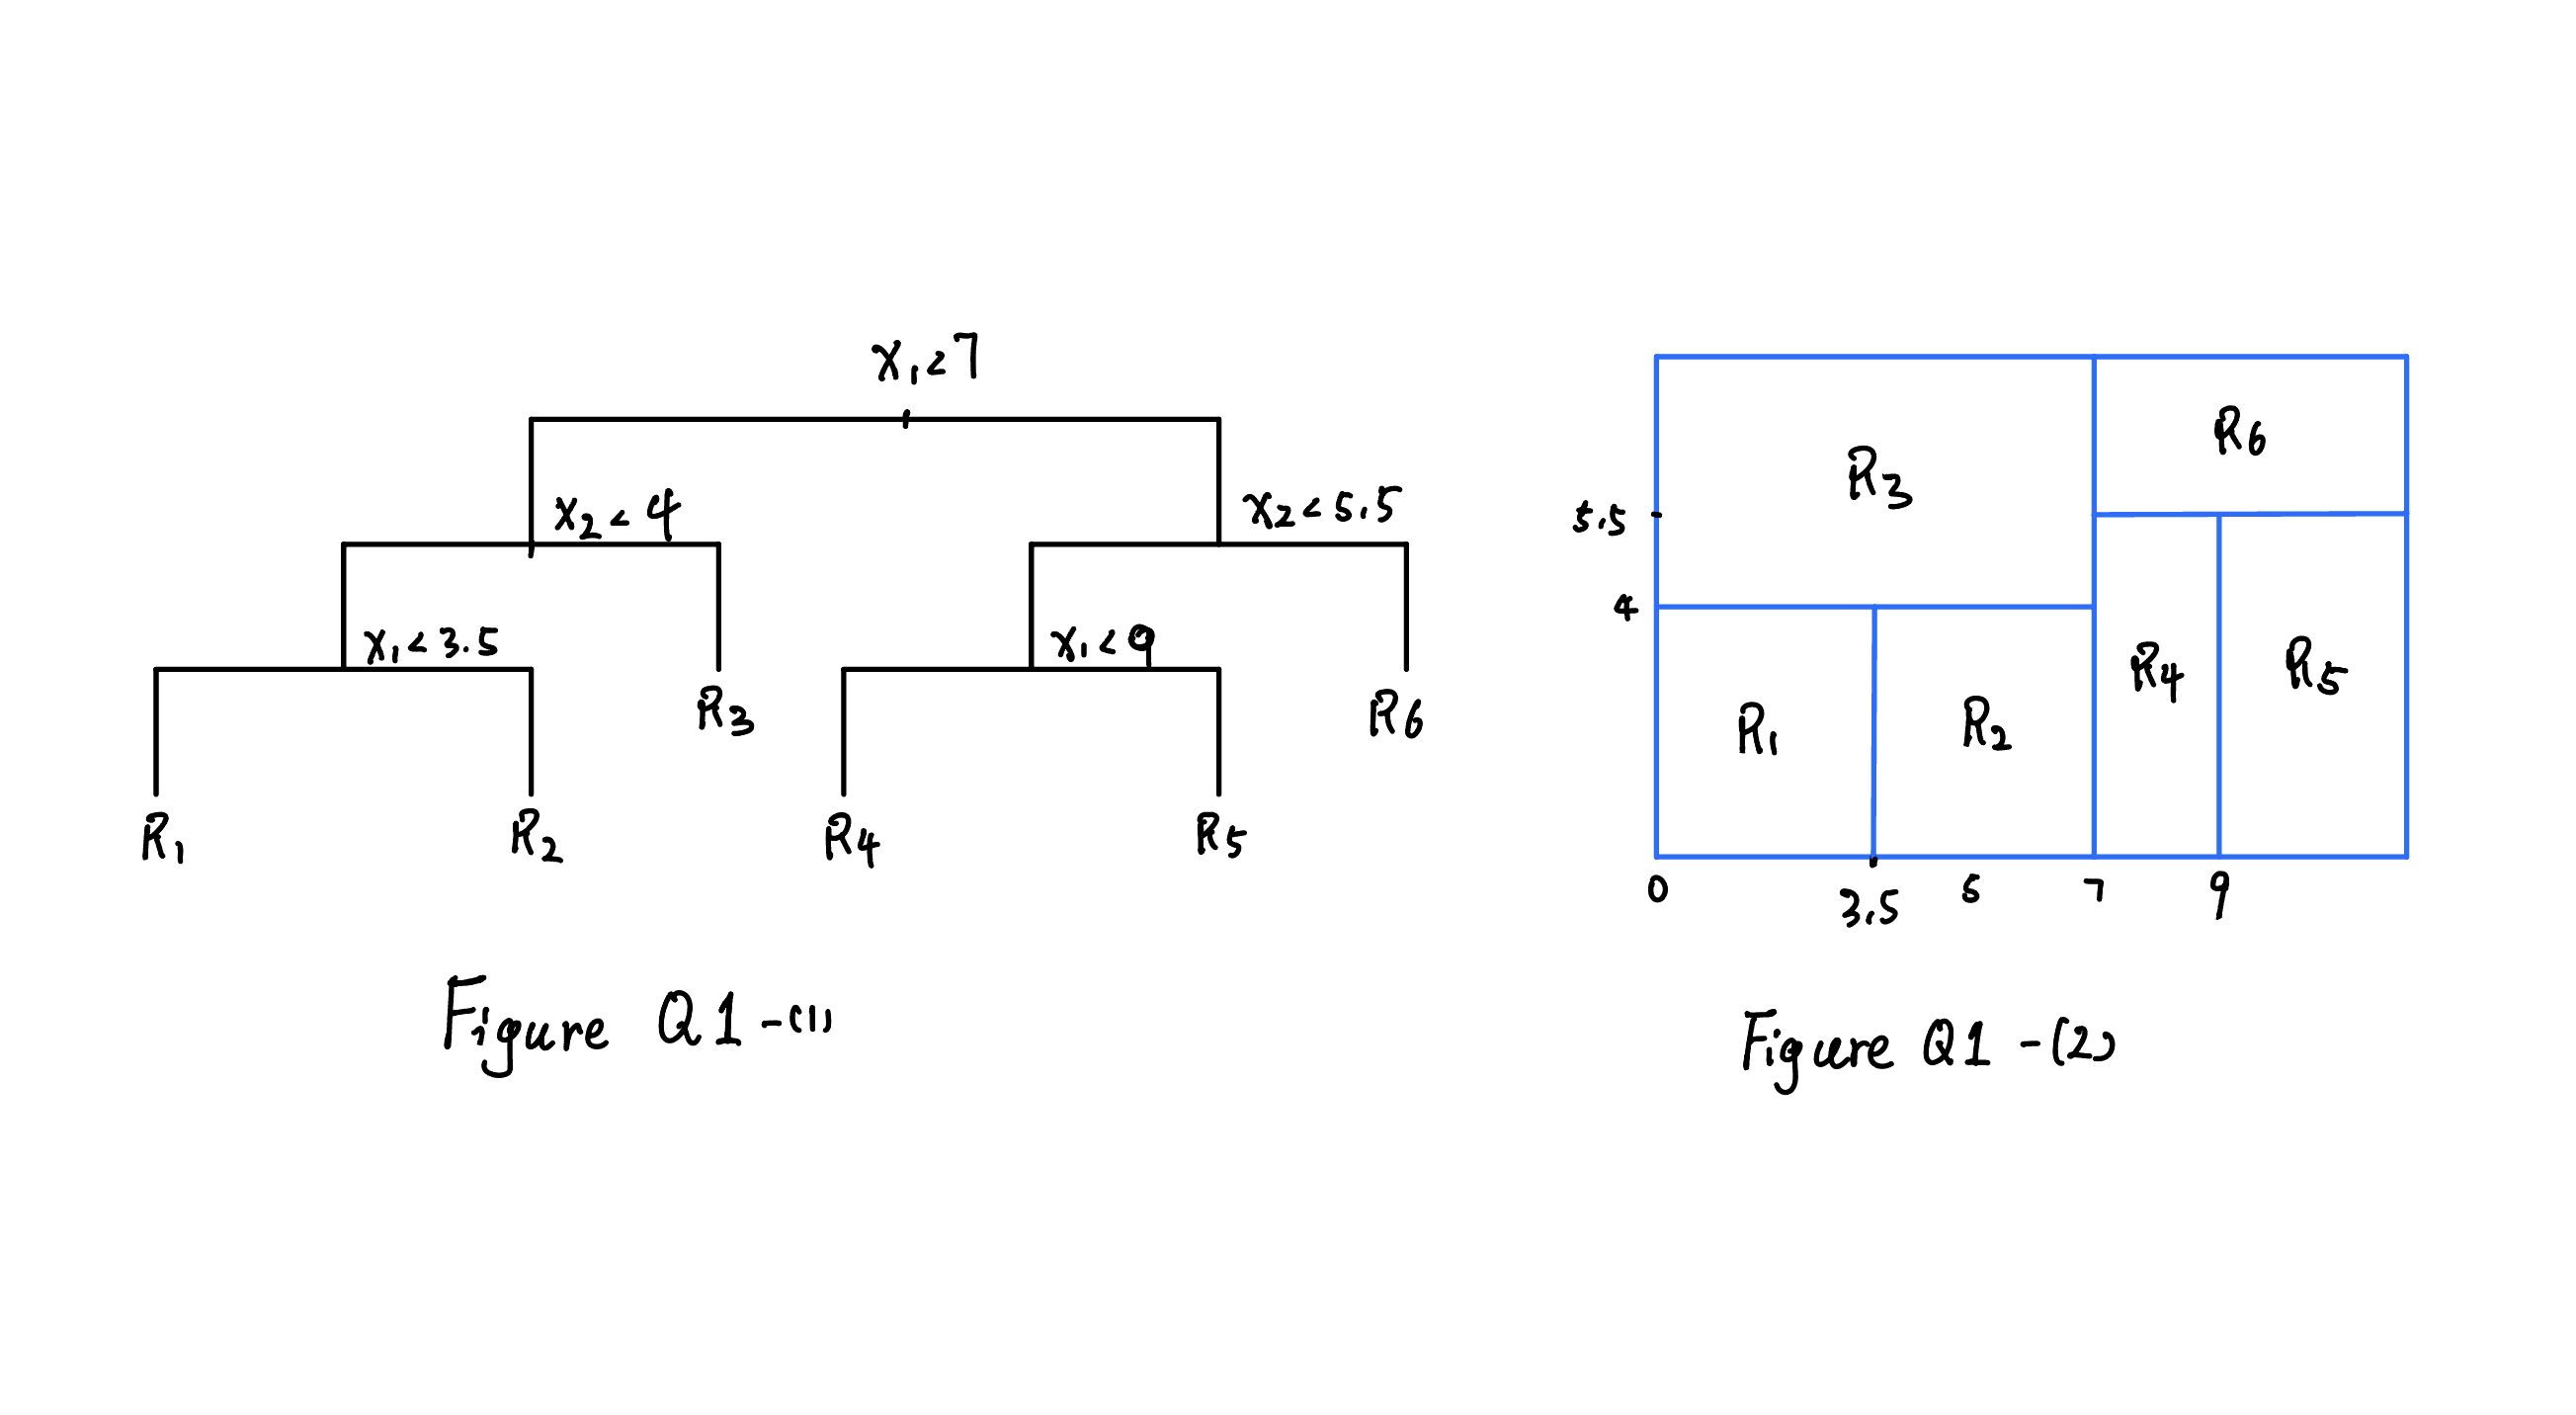
\includegraphics{images/Q1-Figures.jpeg}

\hypertarget{islr_chapter-8-q4}{%
\subsection{2.0 ISLR\_Chapter 8 Q4}\label{islr_chapter-8-q4}}

\emph{This question relates to the plots in Figure 8.14}

\textbf{MY SOLUTION}

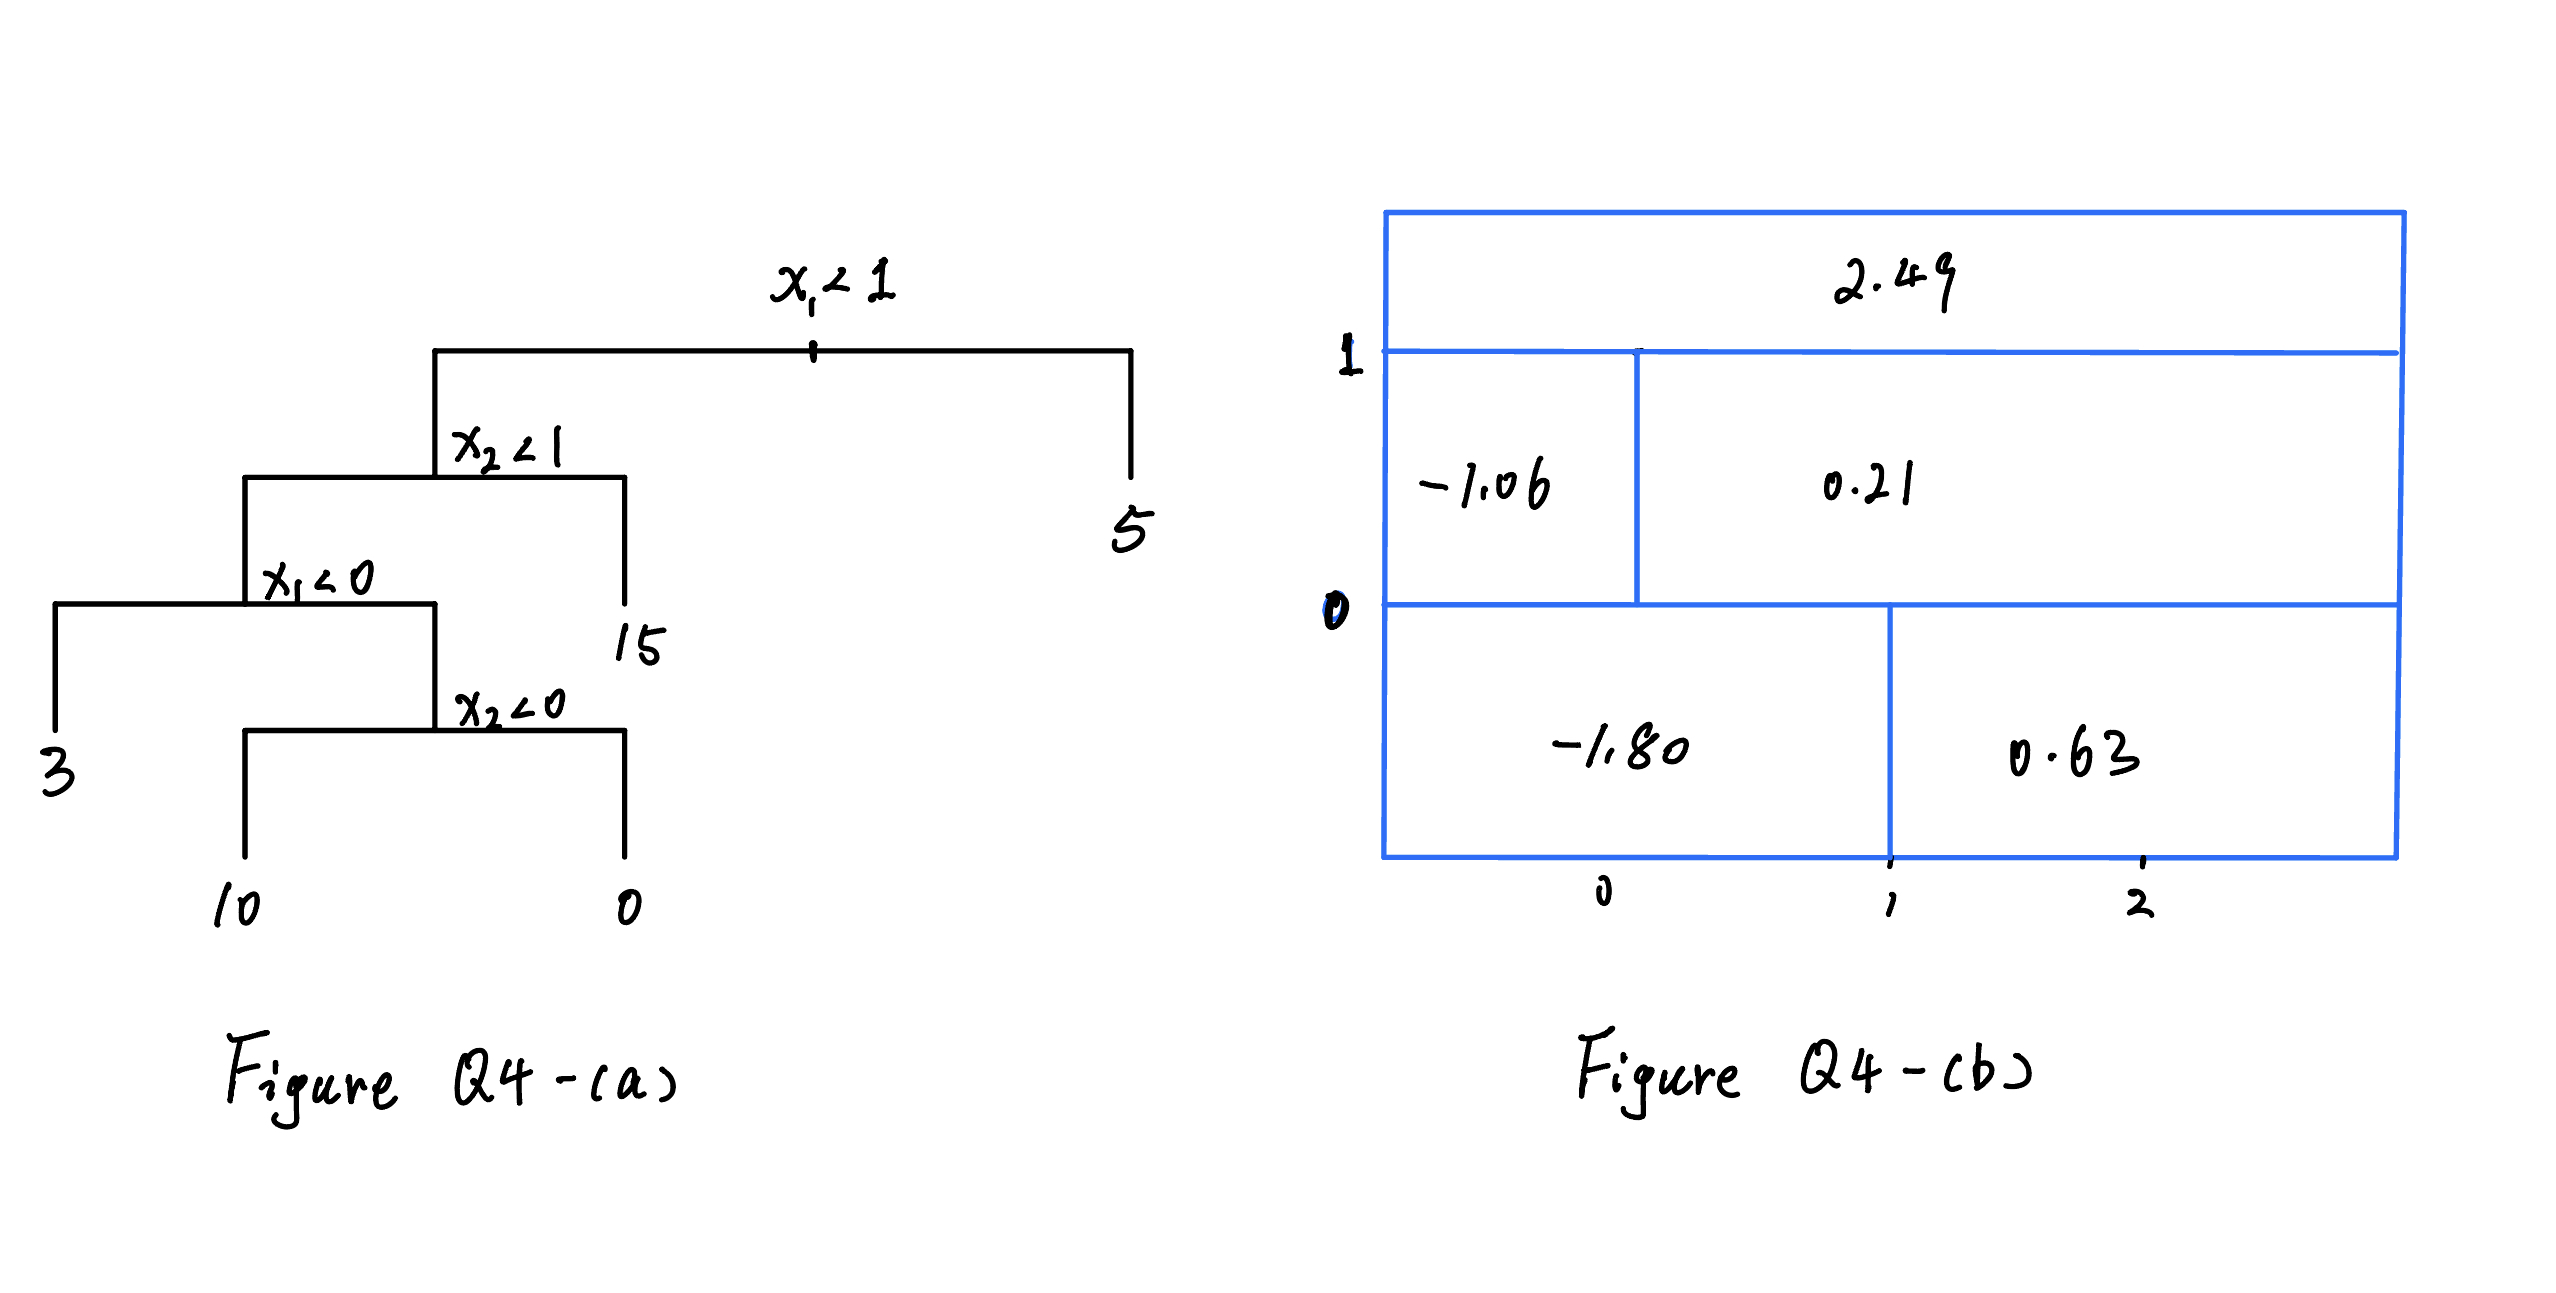
\includegraphics{images/Q4-Figures.jpeg}

\hypertarget{islr_chapter-8-q5}{%
\subsection{3.0 ISLR\_Chapter 8 Q5}\label{islr_chapter-8-q5}}

\emph{Suppose we produce ten bootstrapped samples from a data set
containing red and green classes\ldots.}

\textbf{MY SOLUTION}

For the majority vote method, the class would be red if the probability
is greater than 0.5. Therefore, I counted the number of that, which is
6. Six out of ten predictions indicate that it is the red. Therefore, it
should belong to the red class.

Next, the average probability is 0.45, which is lower than 0.5. Based on
this method, it should be green.

\hypertarget{islr_chapter-8-q6}{%
\subsection{4.0 ISLR\_Chapter 8 Q6}\label{islr_chapter-8-q6}}

\emph{Provide a detailed explanation of the algorithm that is used to
fit a regression tree\ldots.}

\textbf{MY SOLUTION}\\
I seperate the regression tree algorithm into three main stages:

\emph{Stage 1: Tree Growing Stage}

For the regression tree algorithm, one should use the greedy approach
(i.e., recursive binary splitting) to find the best partitioning point
across all data point to split the data into two regions such that the
reduction of RSS is the largest.

We repeat this method on each separated region until each terminal node
has fewer than some minimum number of observations.

\emph{Stage 2: Post-pruning}

Apply the cost complexity pruning to the large tree in order to get a
sequence of best sub-trees, as a function \(\alpha.\)

\emph{Stage 3: CV to find the tuning parameter}

Use K-fold CV to choose \(\alpha.\) Split the training dataset into K
folds and repeat the Stage 1 and 2 on all but the Kth fold. Evaluate the
mean squared prediction error on the data in the left-out Kth fold, as a
function of\(\alpha.\)

Average the results for each value of \(\alpha\), and pick \(\alpha\) to
minimize the average error.

Return the tree calculated using the formula laid out in step 2 on the
entire dataset with that chosen value of \(\alpha\).

\hypertarget{islr_chapter-8-q8}{%
\subsection{5.0 ISLR\_Chapter 8 Q8}\label{islr_chapter-8-q8}}

\emph{We will seek to predict Sales using regression trees and related
approaches, treating the response as a quantitative variable.}

\hypertarget{a}{%
\subsubsection{5.a}\label{a}}

\emph{(a) Split the data set into a training set and a test set.}

\textbf{MY SOLUTION}\\
Here I decided to choose 60\% of the original dataset as a training
part. For the description of the dataset, please see p119 of ISLR2 for
more details.

\begin{Shaded}
\begin{Highlighting}[]
\SpecialCharTok{\textgreater{}} \CommentTok{\# import the data}
\ErrorTok{\textgreater{}} \FunctionTok{library}\NormalTok{(tree)}
\SpecialCharTok{\textgreater{}} \FunctionTok{library}\NormalTok{(ISLR2)}
\SpecialCharTok{\textgreater{}}\NormalTok{ df }\OtherTok{\textless{}{-}}\NormalTok{ Carseats}
\SpecialCharTok{\textgreater{}} 
\ErrorTok{\textgreater{}} \CommentTok{\# randomly select 60\% of the original dataset to be the training. }
\ErrorTok{\textgreater{}}\NormalTok{ train\_index }\OtherTok{\textless{}{-}} \FunctionTok{sample}\NormalTok{(}\DecValTok{1}\SpecialCharTok{:}\FunctionTok{nrow}\NormalTok{(df),}\FunctionTok{nrow}\NormalTok{(df)}\SpecialCharTok{*}\FloatTok{0.6}\NormalTok{)  }
\SpecialCharTok{\textgreater{}}\NormalTok{ df\_train }\OtherTok{\textless{}{-}}\NormalTok{ df[train\_index,]}
\SpecialCharTok{\textgreater{}}\NormalTok{ df\_test }\OtherTok{\textless{}{-}}\NormalTok{ df[}\SpecialCharTok{{-}}\NormalTok{train\_index,]}
\SpecialCharTok{\textgreater{}} \FunctionTok{dim}\NormalTok{(df\_train)}
\NormalTok{[}\DecValTok{1}\NormalTok{] }\DecValTok{240}  \DecValTok{11}
\SpecialCharTok{\textgreater{}} \FunctionTok{dim}\NormalTok{(df\_test)}
\NormalTok{[}\DecValTok{1}\NormalTok{] }\DecValTok{160}  \DecValTok{11}
\end{Highlighting}
\end{Shaded}

This separated datasets look good.

\hypertarget{b}{%
\subsubsection{5.b}\label{b}}

\emph{(b) Fit a regression tree to the training set. Plot the tree, and
interpret the results. What test MSE do you obtain?}

\textbf{MY SOLUTION}

\begin{Shaded}
\begin{Highlighting}[]
\SpecialCharTok{\textgreater{}} \CommentTok{\# fit the model on the training dataset }
\ErrorTok{\textgreater{}}\NormalTok{ model\_tree }\OtherTok{\textless{}{-}} \FunctionTok{tree}\NormalTok{(Sales}\SpecialCharTok{\textasciitilde{}}\NormalTok{., df\_train)}
\SpecialCharTok{\textgreater{}} \FunctionTok{summary}\NormalTok{(model\_tree)}

\NormalTok{Regression tree}\SpecialCharTok{:}
\FunctionTok{tree}\NormalTok{(}\AttributeTok{formula =}\NormalTok{ Sales }\SpecialCharTok{\textasciitilde{}}\NormalTok{ ., }\AttributeTok{data =}\NormalTok{ df\_train)}
\NormalTok{Variables actually used }\ControlFlowTok{in}\NormalTok{ tree construction}\SpecialCharTok{:}
\NormalTok{[}\DecValTok{1}\NormalTok{] }\StringTok{"ShelveLoc"}   \StringTok{"Price"}       \StringTok{"Age"}         \StringTok{"Advertising"} \StringTok{"CompPrice"}  
\NormalTok{[}\DecValTok{6}\NormalTok{] }\StringTok{"Population"} 
\NormalTok{Number of terminal nodes}\SpecialCharTok{:}  \DecValTok{15} 
\NormalTok{Residual mean deviance}\SpecialCharTok{:}  \FloatTok{2.461} \OtherTok{=} \FloatTok{553.7} \SpecialCharTok{/} \DecValTok{225} 
\NormalTok{Distribution of residuals}\SpecialCharTok{:}
\NormalTok{   Min. 1st Qu.  Median    Mean 3rd Qu.    Max. }
\SpecialCharTok{{-}}\FloatTok{3.8280} \SpecialCharTok{{-}}\FloatTok{1.0760}  \FloatTok{0.1077}  \FloatTok{0.0000}  \FloatTok{0.9989}  \FloatTok{6.0010} 
\end{Highlighting}
\end{Shaded}

Next, plot the tree.

\begin{Shaded}
\begin{Highlighting}[]
\SpecialCharTok{\textgreater{}} \FunctionTok{plot}\NormalTok{(model\_tree)}
\SpecialCharTok{\textgreater{}} \FunctionTok{text}\NormalTok{(model\_tree, }\AttributeTok{cex=}\FloatTok{0.5}\NormalTok{,}\AttributeTok{pretty=}\DecValTok{0}\NormalTok{)}
\end{Highlighting}
\end{Shaded}

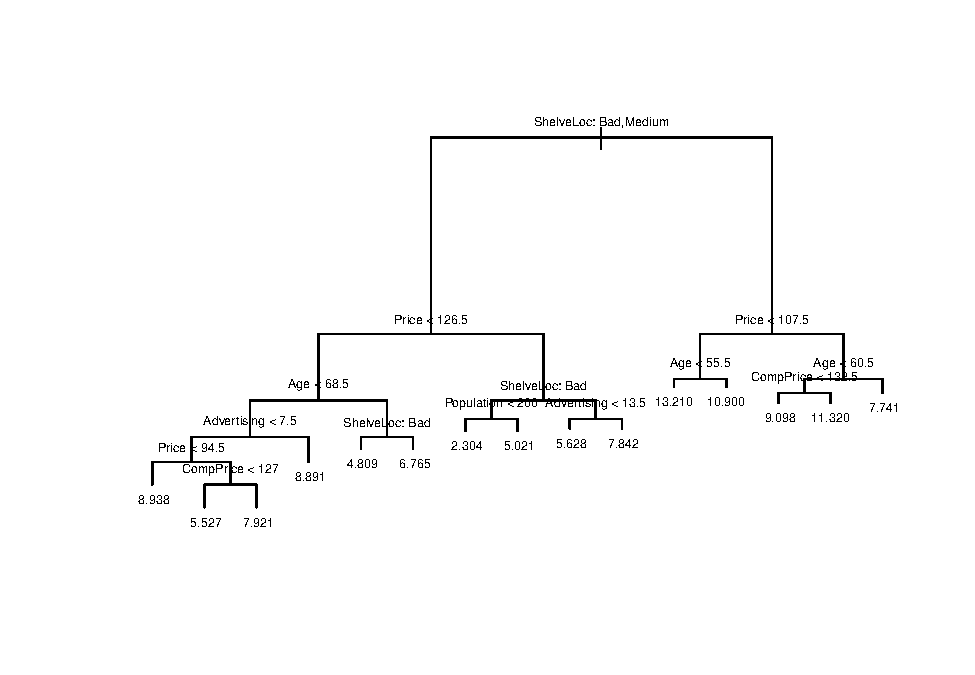
\includegraphics{Homework_13_Pan_files/figure-latex/unnamed-chunk-3-1.pdf}
The plot reveals that the \texttt{ShelveLoc} variable has a significant
impact on car seat sales. Stores with good shelve locations tend to have
higher sales compared to those with medium or bad shelve locations.
Additionally, the plot suggests that price plays a crucial role in
customer behavior as they appear to be price-sensitive. Specifically,
lower prices are associated with higher sales.

Next, to get the MSE.

\begin{Shaded}
\begin{Highlighting}[]
\SpecialCharTok{\textgreater{}}\NormalTok{ model\_pred }\OtherTok{\textless{}{-}} \FunctionTok{predict}\NormalTok{(model\_tree, }\AttributeTok{newdata=}\NormalTok{df\_test)}
\SpecialCharTok{\textgreater{}}\NormalTok{ (mse\_ }\OtherTok{\textless{}{-}} \FunctionTok{round}\NormalTok{(}\FunctionTok{mean}\NormalTok{((model\_pred}\SpecialCharTok{{-}}\NormalTok{df\_test}\SpecialCharTok{$}\NormalTok{Sales)}\SpecialCharTok{\^{}}\DecValTok{2}\NormalTok{),}\DecValTok{3}\NormalTok{))}
\NormalTok{[}\DecValTok{1}\NormalTok{] }\FloatTok{4.807}
\end{Highlighting}
\end{Shaded}

The MSE is 4.807.

\hypertarget{c}{%
\subsubsection{5.c}\label{c}}

\emph{(c) Use cross-validation in order to determine the optimal level
of tree complexity}

\textbf{MY SOLUTION}

\begin{Shaded}
\begin{Highlighting}[]
\SpecialCharTok{\textgreater{}}\NormalTok{ model\_cv }\OtherTok{\textless{}{-}} \FunctionTok{cv.tree}\NormalTok{(model\_tree)}
\SpecialCharTok{\textgreater{}} \CommentTok{\# par(mfrow=c(1,2))}
\ErrorTok{\textgreater{}} \FunctionTok{plot}\NormalTok{(model\_cv}\SpecialCharTok{$}\NormalTok{size, model\_cv}\SpecialCharTok{$}\NormalTok{dev, }\AttributeTok{type =} \StringTok{"l"}\NormalTok{)}
\end{Highlighting}
\end{Shaded}

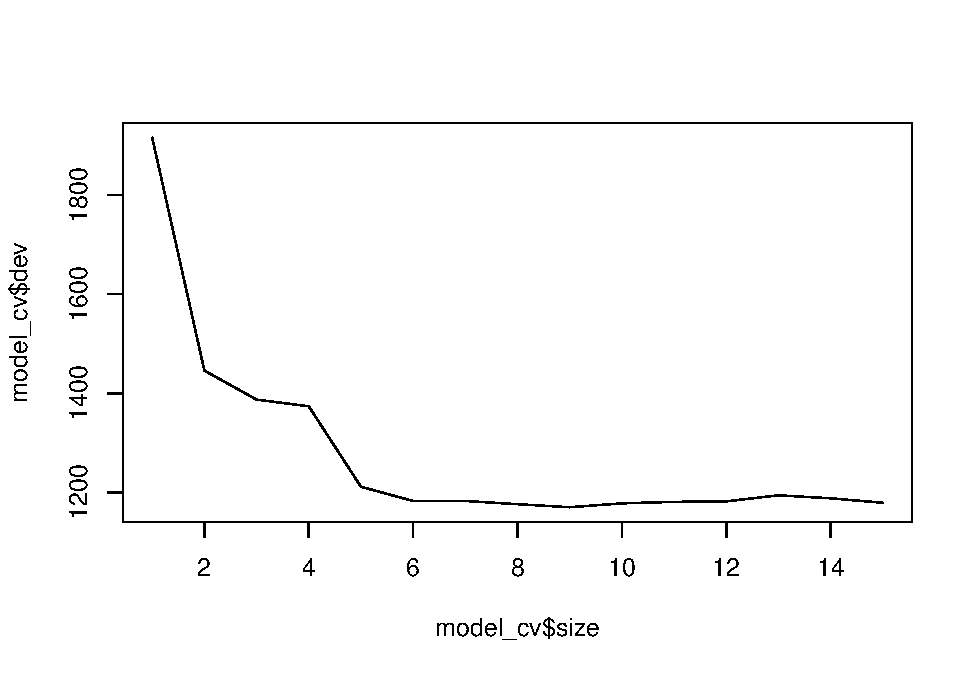
\includegraphics{Homework_13_Pan_files/figure-latex/unnamed-chunk-5-1.pdf}
Note, the function \texttt{cv.tree()} returns the \texttt{dev} to
represent the error rate and the \texttt{k} to indicate the tuning
parameter \(\alpha\). From the results, the 6 is the best size.

\begin{Shaded}
\begin{Highlighting}[]
\SpecialCharTok{\textgreater{}}\NormalTok{ model\_prune }\OtherTok{\textless{}{-}} \FunctionTok{prune.tree}\NormalTok{(model\_tree, }\AttributeTok{best =} \DecValTok{6}\NormalTok{)}
\SpecialCharTok{\textgreater{}} \FunctionTok{plot}\NormalTok{(model\_prune)}
\SpecialCharTok{\textgreater{}} \FunctionTok{text}\NormalTok{(model\_prune, }\AttributeTok{cex=}\FloatTok{0.5}\NormalTok{,}\AttributeTok{pretty=}\DecValTok{0}\NormalTok{)}
\end{Highlighting}
\end{Shaded}

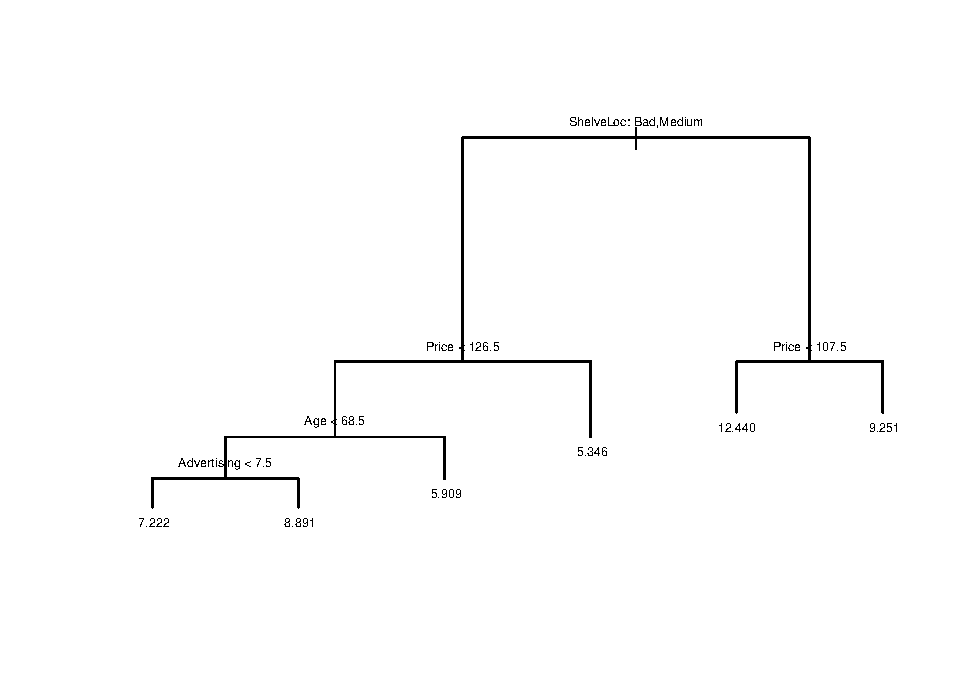
\includegraphics{Homework_13_Pan_files/figure-latex/unnamed-chunk-6-1.pdf}

\begin{Shaded}
\begin{Highlighting}[]
\SpecialCharTok{\textgreater{}}\NormalTok{ model\_prune\_pred }\OtherTok{\textless{}{-}} \FunctionTok{predict}\NormalTok{(model\_prune, }\AttributeTok{newdata=}\NormalTok{df\_test)}
\SpecialCharTok{\textgreater{}}\NormalTok{ (mse\_2 }\OtherTok{\textless{}{-}} \FunctionTok{round}\NormalTok{(}\FunctionTok{mean}\NormalTok{((model\_prune\_pred}\SpecialCharTok{{-}}\NormalTok{df\_test}\SpecialCharTok{$}\NormalTok{Sales)}\SpecialCharTok{\^{}}\DecValTok{2}\NormalTok{),}\DecValTok{3}\NormalTok{))}
\NormalTok{[}\DecValTok{1}\NormalTok{] }\FloatTok{5.017}
\end{Highlighting}
\end{Shaded}

This time, the pruned model make the MSE worse. The MSE for pruned tree
is 5.017, and for the unpruned tree is 4.807.

\end{document}
